\documentclass[11pt,a4paper]{article}
\usepackage[utf8]{inputenc}
\usepackage[T1]{fontenc}
\usepackage[spanish,es-noquoting,es-nodecimaldot]{babel}
\usepackage{amsmath,amssymb,bm,slashed}
\usepackage{booktabs,longtable}
\usepackage{graphicx}
\usepackage[margin=2.3cm]{geometry}
\usepackage[colorlinks=true,linkcolor=blue!60!black,citecolor=blue!60!black,urlcolor=blue!60!black]{hyperref}
\usepackage{xcolor}
\newcommand{\Ap}{A'}
\newcommand{\eps}{\epsilon}
\newcommand{\KN}{\mathrm{KN}}
\newcommand{\dd}{\mathrm{d}}
\newcommand{\verdict}[1]{\textbf{\color{red!70!black}#1}}
\newcommand{\ok}[1]{\textbf{\color{green!50!black}#1}}
\title{La sección eficaz de producción de fotones oscuros en un reactor\\[2pt]
\large Clase 1: una fórmula exacta, tres apuntes, ocho papers, y qué diferencias son errores}
\author{E.~L.~De Paoli\\[2pt]\small escrito con asistencia de agentes (Claude Opus 5)}
\date{21 de septiembre de 2026}

\begin{document}
\maketitle

\begin{abstract}
\noindent\sloppy
Los documentos de \texttt{apuntes/} no calculan lo mismo. El apunte en castellano
(\texttt{Dark\_Photon\_cross\_section-1.pdf}) deriva la sección eficaz a nivel árbol de $\gamma e^-\to \Ap e^-$ y el caso
con masa le sale mal: la amplitud al cuadrado, la cinemática y el rango cinemático tienen errores, y su
$\dd\sigma/\dd E_{\Ap}$ final se aparta hasta un factor 2 punto a punto y cruza un polo de propagador dentro de su propio
rango de integración para $m_{\Ap}=1$~MeV. Cada error tiene una corrección de una línea (Sección~\ref{sec:note}). El
informe \emph{v2} (\texttt{report\_park\_production\_v2}) tiene la sección eficaz a nivel árbol exactamente bien: la
rederivé con matrices de Dirac explícitas y coincide con la fórmula del \emph{v2}, con deNiverville--Lee--Lee y con
Smirnov et al.\ a $2\times10^{-13}$. Su convolución con el espectro del reactor, en cambio, no es lo que da la ecuación de
fuente de Park: tanto la Figura~2 del \emph{v2} como la Figura~1 de Park tienen una cola igual al espectro de fotones,
mientras que la convolución tipo Compton es 4--8 veces menor por encima de 2~MeV. El informe \emph{v3}
(\texttt{report\_darkphoton\_v3}) usa un mecanismo distinto (oscilación en el medio, Danilov et al.); no es otra forma de
hacer el mismo cálculo, es el canal de producción dominante, y la fórmula de Park lo omite. En la ventana 3--8~MeV de
TEXONO los dos mecanismos difieren en un factor $7.7$ al mismo $\eps$ (Figura~\ref{fig:two}). El factor $2/3$ de detección
de Park es el promedio no polarizado y es incorrecto para el haz que un reactor produce; el factor correcto es $\approx1$
para $m_{\Ap}\lesssim0.1$~MeV y está entre $0.8$ y $1$ hasta 1~MeV.
\end{abstract}

\section{La pregunta}
Se piden tres cosas. (i)~¿Difieren los documentos de \texttt{apuntes/} en el enfoque teórico de la sección eficaz?
(ii)~¿Difieren las fórmulas \emph{finales}, las que hacen falta para el número de fotones oscuros que llegan a un
detector? (iii)~¿Las diferencias vienen de errores? Las respuestas: sí; sí; y casi todas sí, con una excepción que no es
un error sino una omisión de física.

Todo lo numérico de abajo lo produjo \texttt{work/check\_cross\_section.py} (cada bloque termina en un \texttt{assert}) y
\texttt{work/figures\_cross\_section.py} (marimo). El recibo de ejecución está en la Sección~\ref{sec:receipt}. En cada
paso digo qué derivé y qué recordé.

\section{Planteo}
Proceso, notación e interacción (recordado, estándar):
\begin{equation}
\gamma(k)+e^-(p)\to \Ap(q)+e^-(p'),\quad m\equiv m_e,\; M\equiv m_{\Ap},\quad
\mathcal L_{\rm int}=-e\,\bar\psi\gamma^\mu\psi\,(A_\mu+\eps A'_\mu),\quad e^2=4\pi\alpha .
\end{equation}
El electrón es libre y está en reposo. Dos diagramas árbol (intercambio de electrón en canal $s$ y $u$). Invariantes:
\begin{equation}
s=(p+k)^2=m^2+2mE,\qquad u=(p-q)^2=m^2+M^2-2mx,\qquad t=(p-p')^2=2m(x-E),
\end{equation}
con $E$ la energía del fotón y $x$ la energía del $\Ap$ en el laboratorio. Uso los denominadores de propagador
\begin{equation}
a\equiv s-m^2=2mE,\qquad b\equiv u-m^2=M^2-2mx,\qquad c\equiv m^2,\qquad d\equiv M^2 .
\label{eq:abcd}
\end{equation}

\section{Cinemática (derivada, exacta)}
De $(p+k-q)^2=m^2$ con $Q=|\vec q|=\sqrt{x^2-M^2}$:
\begin{equation}
M^2+2m(E-x)-2E\,(x-Q\cos\theta)=0
\quad\Longrightarrow\quad
\cos\theta=\frac{(x-m)E+mx-M^2/2}{EQ}.
\label{eq:costheta}
\end{equation}
Es trascendente en $x$ a $\theta$ fijo porque $Q\neq x$. Los extremos de $x$ salen del impulso de dos cuerpos en el CM
llevado al laboratorio:
\begin{equation}
x_\pm=\frac{(E+m)(s+M^2-m^2)\pm E\sqrt{\lambda(s,m^2,M^2)}}{2s},\qquad
\lambda(s,m^2,M^2)=[s-(m+M)^2][s-(m-M)^2],
\label{eq:xpm}
\end{equation}
y el umbral es $s\ge (m+M)^2$:
\begin{equation}
E_{\rm th}=M+\frac{M^2}{2m}\;:\qquad 0.1098,\;0.7446,\;1.9785~\text{MeV para }M=0.1,\,0.5,\,1~\text{MeV}.
\label{eq:thr}
\end{equation}
El umbral \emph{no} es $E=M$. A $M=1$~MeV es el doble.

\section{La amplitud al cuadrado (derivada dos veces)}
Con $\Gamma^{\nu\mu}=\gamma^\nu(\slashed r_s+m)\gamma^\mu/a+\gamma^\mu(\slashed r_u+m)\gamma^\nu/b$,
$r_s=p+k$, $r_u=p-q$, la amplitud es $\mathcal M=\eps e^2\,\bar u(p')\Gamma^{\nu\mu}u(p)\,\varepsilon_\mu(k)\xi^*_\nu(q)$.
Promediando sobre las dos polarizaciones del fotón y los dos espines del electrón, sumando sobre espines finales y las
tres polarizaciones del $\Ap$:
\begin{equation}
\overline{|\mathcal M|^2}=\eps^2e^4\,F,\qquad
\boxed{\;F=-2\Big(\frac ab+\frac ba\Big)+4(2c+d)\Big[\Big(\frac1a+\frac1b\Big)+c\Big(\frac1a+\frac1b\Big)^2-\frac{d}{ab}\Big]\;}
\label{eq:F}
\end{equation}
Es la ec.~(36) del informe \emph{v2}. No la tomé por buena. Mi chequeo construye las matrices de Dirac $4\times4$, los
vectores de polarización explícitos (dos para el fotón, $\varepsilon_{1,2}$; tres para el $\Ap$, incluido
$\xi_L=(Q,\,x\hat q)/M$), arma $\Gamma$ numéricamente y evalúa
$\tfrac14\sum\mathrm{Tr}[(\slashed p'+m)\Gamma(\slashed p+m)\bar\Gamma]$ en 60 puntos aleatorios on-shell del laboratorio con
$M\in[0.05,1.5]$~MeV, $E\le10$~MeV. No se usa ninguna identidad de trazas. Resultados:
\begin{itemize}
\item suma explícita sobre polarizaciones $=$ suma covariante $(-g_{\mu\mu'})(-g_{\nu\nu'})$ a $2\times10^{-13}$ (vale la
identidad de Ward $q_\nu\mathcal M^\nu=0$, así que el término $q_\nu q_{\nu'}/M^2$ cae);
\item numérico $=$ ec.~\eqref{eq:F} a $2\times10^{-13}$;
\item numérico $=$ deNiverville--Lee--Lee ecs.~(18)--(20) a $2\times10^{-13}$;
\item $\dd\sigma/\dd x$ de la ec.~\eqref{eq:F} $=$ Smirnov et al.\ ec.~(3) (con $Z=1$, $g_X=\eps e$, $x_S=1-x/E+M^2/2mE$)
a $9\times10^{-16}$.
\end{itemize}
Tres formas publicadas independientes y un cálculo con matrices explícitas coinciden. La ec.~\eqref{eq:F} es la
sección eficaz a nivel árbol. En $d=0$ es Klein--Nishina, $F=2\,[x/E+E/x-\sin^2\theta]$ (verificado con sympy).

\section{Secciones eficaces}
Recordado: $\dd\sigma/\dd t=\overline{|\mathcal M|^2}/[16\pi(s-m^2)^2]$. Derivado: $\dd t/\dd x=2m$. Entonces
\begin{equation}
\boxed{\;\frac{\dd\sigma}{\dd x}=\frac{\eps^2e^4}{32\pi\,m\,E^2}\,F(a,b,c,d),\qquad a=2mE,\; b=M^2-2mx,\quad x\in[x_-,x_+]\;}
\label{eq:dsdx}
\end{equation}
Total: $\sigma=\int_{x_-}^{x_+}\dd x\,\dd\sigma/\dd x$; la forma cerrada $G(b)$ del \emph{v2} (su ec.~41) cumple
$\dd G/\dd b=F$ (verificado simbólicamente). La cuadratura de la ec.~\eqref{eq:dsdx} en $M\to0$ reproduce $\sigma_\KN$ en
$E=1,3,8$~MeV a $10^{-6}$. Supresión por masa en $E=3$~MeV:
$\sigma/\sigma_\KN=0.995,\,0.886,\,0.609$ para $M=0.1,\,0.5,\,1$~MeV.

\begin{figure}[t]\centering
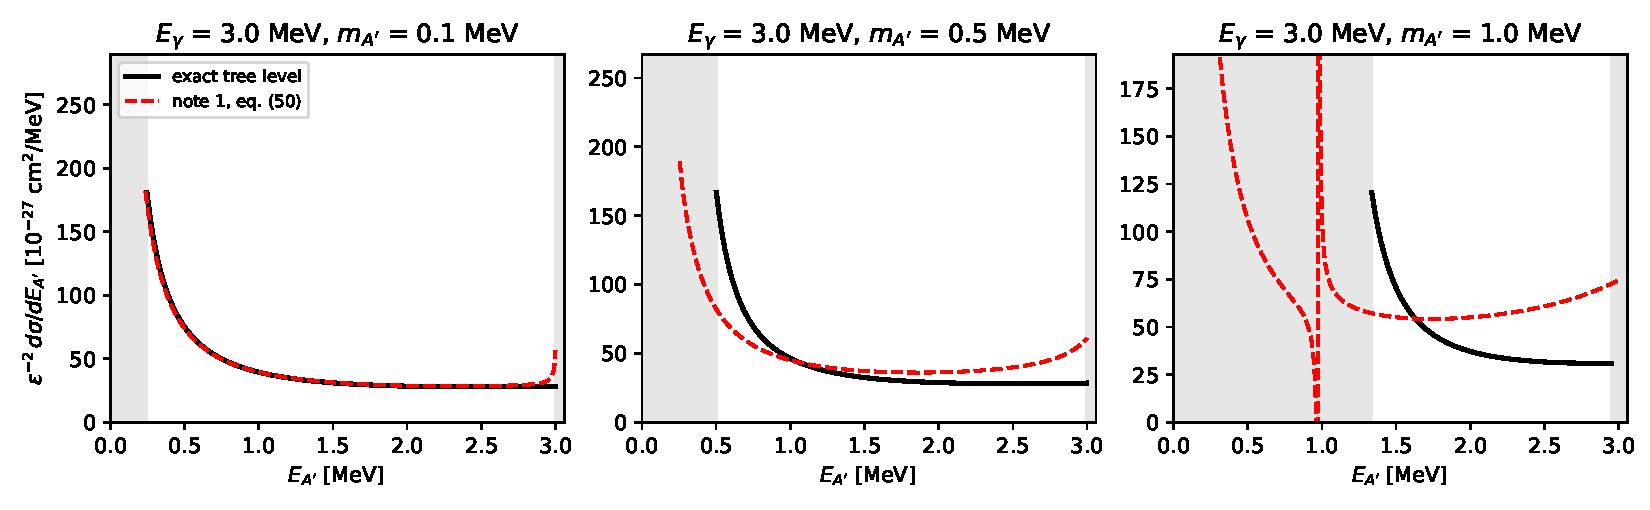
\includegraphics[width=\textwidth]{../work/fig_dsigma_dx_E3.pdf}
\caption{$\eps^{-2}\dd\sigma/\dd E_{\Ap}$ en $E_\gamma=3$~MeV. Negro: ec.~\eqref{eq:dsdx}. Rojo a trazos: ec.~(50) del
apunte, dibujada sobre el rango que el propio apunte declara. Gris: fuera del rango exacto $[x_-,x_+]$. En $M=1$~MeV la
fórmula del apunte tiene un polo en $E_{\Ap}=M^2/2m=0.978$~MeV ($u-m^2=0$) dentro de su propio rango.}
\label{fig:dsdx}
\end{figure}

\section{El apunte en castellano: qué está mal y cómo corregirlo}
\label{sec:note}
\texttt{Dark\_Photon\_cross\_section-1.pdf} (se omite el nombre del autor) sigue el camino correcto: reglas de Feynman $\to$ traza $\to$
espacio de fases en el laboratorio. Su total en $M=0$ (ec.~52) está bien y coincide idénticamente con Klein--Nishina
(verificado con sympy). Todo lo que depende de $M\neq0$ necesita las correcciones de abajo. Los errores se acumulan:
$|\mathcal M|^2$ mal $\times$ jacobiano mal $\times$ rango mal.

{\small
\begin{longtable}{@{}p{2.3cm}p{4.2cm}p{3.9cm}p{4.6cm}@{}}
\toprule
Ítem & El apunte dice & Qué está mal & Corrección \\
\midrule
\endhead
Cinemática, ecs.~(17)--(19) & resuelve $M^2+2m(\omega-\omega')-2\omega\omega'(1-\cos\theta)=0$, o sea $|\vec k'|\approx\omega'$;
$\omega'=\frac{\omega+M^2/2m}{1+\frac{\omega}{m}(1-\cos\theta)}$ &
El álgebra está bien (la ec.~19 sí resuelve la ec.~18) pero la ec.~18 misma es una aproximación. En $E=3$, $x=2$,
$M=1$~MeV da $\cos\theta=0.832$; el exacto es $0.960$. &
Conservar $|\vec k'|=\sqrt{\omega'^2-M^2}$: reemplazar la ec.~(18) por la ec.~\eqref{eq:costheta}. Trabajar en
$\omega'$, no en $\theta$; la relación es trascendente en $\omega'$ y no hace falta invertirla.\\
Umbral, Cuadro~1 & $\omega\to M$ & Mal: el estado final tiene que llevarse el impulso del fotón, y eso cuesta $M^2/2m$.
El Cuadro~1 no se usa en la derivación de la ec.~(50), así que por sí sola esta entrada es inocua; el mismo error entra
por el rango, fila siguiente. & $E_{\rm th}=M+M^2/2m$, ec.~\eqref{eq:thr}: $1.98$~MeV para $M=1$~MeV, no $1$~MeV.\\
Rango, ecs.~(24)--(25) & $\omega'\in\big[\frac{m\omega+M^2/2}{2\omega+m},\,\omega\big]$ &
Mal en los dos extremos: $\omega'=\omega$ es imposible con $M\neq0$, y el extremo inferior queda por debajo del
verdadero. $E=3$, $M=1$: exacto $[1.336,2.955]$, apunte $[0.312,3.000]$. Este rango es no vacío para todo $\omega\ge M/2$,
y con $\omega'\ge M$ da $\omega\ge M$: es el umbral ingenuo del Cuadro~1 disfrazado, y esta copia \emph{sí} se usa al
integrar la ec.~(50). &
Usar $x_\pm$ de la ec.~\eqref{eq:xpm} (boost del impulso en el CM). Para $M\to0$ se reduce a los límites del apunte.\\
$\overline{|\mathcal M|^2}$, ecs.~(35)--(40) & $2\eps^2e^4\big[-\frac us-\frac su+2M^2(\frac1s+\frac1u)-\frac{M^4}{4}(\frac1s+\frac1u)^2su\big]$
($s,u$ = denominadores de propagador) &
De $-39\%$ a $+33\%$ contra la ec.~\eqref{eq:F}. Las ecs.~(35)--(36) descartan los términos en $m^2$ como
``$O(m_e^2/s)$'', pero $m_e^2/s$ no es chico a energías de MeV: en $M=0$ falta exactamente
$8m^2(\frac1a+\frac1b)+8m^4(\frac1a+\frac1b)^2$, que es lo que produce el $-\sin^2\theta$ de Klein--Nishina. La
ec.~(39) no es la traza que nombra. &
Reemplazar la ec.~(40) por la ec.~\eqref{eq:F} con $a=s$, $b=u$ en la notación del apunte. Conservar todas las
potencias de $m$; en este problema no hay ningún régimen con $m_e\ll\sqrt s$.\\
$\dd\sigma/\dd\Omega$, ecs.~(43)--(46) & corchete KN $+M^2 f(s,u)$, $f=\frac{2}{s+u}(1-\frac{m^2M^2}{su})$, factor de
espacio de fases sin masa $(\omega'/\omega)^2$ &
No se sigue de la ec.~(40): el término $-\sin^2\theta$ necesita los términos en $m^2$ descartados antes. El factor de
espacio de fases para una partícula final masiva lleva $|\vec k'|\omega'$, no $\omega'^2$. &
No pasar por $\dd\Omega$. Usar la forma invariante $\dd\sigma/\dd t=\overline{|\mathcal M|^2}/[16\pi(s-m^2)^2]$ y
$\dd t=2m\,\dd\omega'$; eso da la ec.~\eqref{eq:dsdx} sin ningún jacobiano angular.\\
Jacobiano, ecs.~(47)--(48) & $\dd\Omega/\dd\omega'=\frac{2\pi}{\omega'^2}(m+\frac{M^2}{2\omega})$ &
Derivado de la ec.~(20) aproximada; el exacto tiene $|\vec k'|$ adentro. & No hace falta una vez que se usa la
ec.~\eqref{eq:dsdx}.\\
$\dd\sigma/\dd\omega'$ final, ec.~(50) & $\frac{\pi\eps^2\alpha^2}{m\omega^2}(1+\frac{M^2}{2m\omega})[\ldots]$ &
Hasta $2\times$ de error punto a punto (Fig.~\ref{fig:dsdx}); tiene un polo en $\omega'=M^2/2m$ ($u=0$ en la notación
del apunte) que cae dentro del rango del apunte para $M=1$~MeV ($0.978\in[0.312,3]$), así que ahí el total no existe.
Sobre el rango exacto el total queda $0.5\%$, $7\%$, $36\%$ alto para $M=0.1$, $0.5$, $1$~MeV. &
Ec.~\eqref{eq:dsdx} sobre $[x_-,x_+]$. El polo queda fuera del rango exacto para todo $M<2m$.\\
\bottomrule
\end{longtable}}

\paragraph{Cuál de estos errores pesa en el número de fotones oscuros.} Convolucionando la ec.~(50) del apunte, sobre el
rango del apunte, con el espectro de Park mediante la ec.~\eqref{eq:park1} ($\sigma_{\rm tot}=\sigma_\KN$, 1~GW, $\eps=1$) y
comparando con la misma convolución de la ec.~\eqref{eq:dsdx} sobre $[x_-,x_+]$ (\texttt{work/check\_eq50\_fold.py}):
\begin{center}\small
\begin{tabular}{@{}lcccc@{}}
\toprule
$M$ [MeV] & fotones con $M<\omega<E_{\rm th}$ & \multicolumn{2}{c}{$\dd\dot N/\dd E_{\Ap}$, apunte/exacto} & $\dot N_{\Ap}$(3--8~MeV), apunte/exacto\\
 & & en 3~MeV & en 5~MeV & \\
\midrule
0.1 & 1.1\% & 1.06 & 1.05 & 1.05\\
0.5 & 23.6\% & 1.48 & 1.43 & 1.46\\
1.0 & 65.9\% & 2.05 & 1.90 & 1.99\\
\bottomrule
\end{tabular}
\end{center}
En la ventana 3--8~MeV el error de umbral/rango no aporta nada: un $\Ap$ de $E_{\Ap}\ge3$~MeV viene de un fotón de
$\omega\ge3$~MeV, y todos esos están sobre el umbral para $M\le1$~MeV ($\omega'_{\max}=\omega$ en vez de $x_+$ mueve la
energía mínima del fotón de $3$ a $3.05$~MeV). Los factores $1.05$, $1.46$, $1.99$ vienen de la ec.~(50) misma: el
$|\mathcal M|^2$ sin sus términos en $m^2$ y el jacobiano sin masa. Ese es el error a corregir para el CsI de TEXONO.
El error de rango pesa a baja $E_{\Ap}$: para $M=1$~MeV, el $66\%$ de los fotones por encima de $1$~MeV está bajo el
umbral verdadero y el apunte los deja producir $\Ap$; para $E_{\Ap}$ entre $0.31$ y $1.34$~MeV la ec.~(50) integra sobre
una región cinemáticamente prohibida que contiene el polo en $0.978$~MeV (en $E_{\Ap}=1$~MeV: exacto $0$, apunte
$1.5\times10^{21}$~MeV$^{-1}$s$^{-1}$). Eso importa para un detector de umbral bajo como el PCGe de TEXONO, no para el CsI.

\paragraph{Corrección mínima de la ec.~(50).} Reemplazar el corchete $[\ldots]$ por $F/2$ con $a=2m\omega$,
$b=M^2-2m\omega'$, $c=m^2$, $d=M^2$; reemplazar el prefactor $\frac{\pi\eps^2\alpha^2}{m\omega^2}(1+\frac{M^2}{2m\omega})$
por $\frac{\pi\eps^2\alpha^2}{m\omega^2}$, o sea $\dd\sigma/\dd\omega'=\eps^2e^4F/(32\pi m\omega^2)$; reemplazar el rango
por $[x_-,x_+]$. El umbral sale solo y el polo queda fuera del rango para todo $M<2m$.

\noindent Con esos reemplazos el resumen de la Sección~9 del apunte queda: $\cos\theta$ de la ec.~\eqref{eq:costheta},
$\overline{|\mathcal M|^2}=\eps^2e^4F$ con la ec.~\eqref{eq:F}, $\dd\sigma/\dd\omega'$ de la ec.~\eqref{eq:dsdx}, rango
$[x_-,x_+]$ de la ec.~\eqref{eq:xpm}, umbral ec.~\eqref{eq:thr}. Su Sección~8 (el total en $M=0$) queda como está.

\begin{figure}[t]\centering
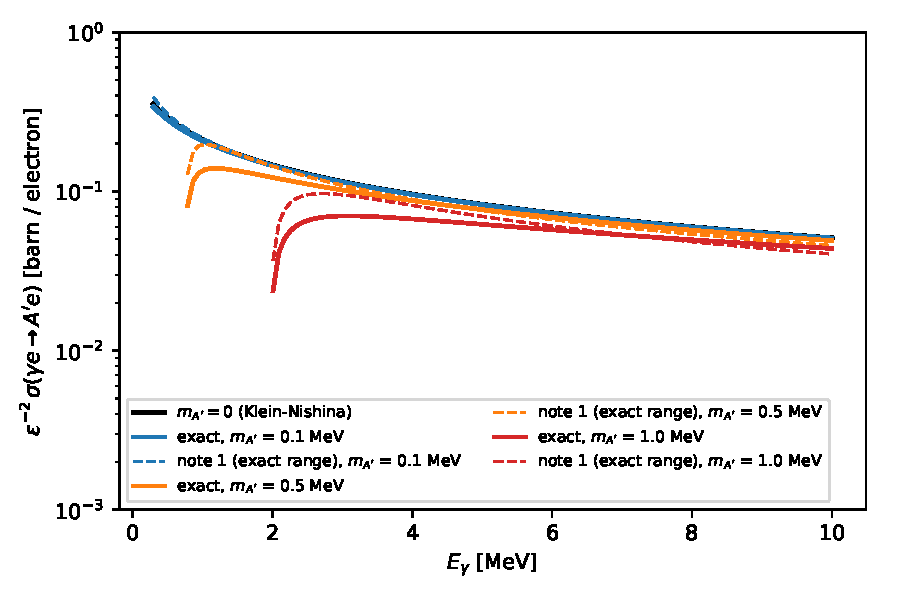
\includegraphics[width=0.62\textwidth]{../work/fig_sigma_total.pdf}
\caption{Sección eficaz total de producción por electrón, $\eps=1$. Línea llena: ec.~\eqref{eq:dsdx} integrada sobre
$[x_-,x_+]$; la curva $M=0$ es Klein--Nishina. A trazos: el integrando del apunte integrado sobre el rango
\emph{exacto} (sobre su propio rango diverge para $M=1$~MeV).}
\end{figure}

\section{El informe v2: correcto, y qué no resuelve}
\texttt{report\_park\_production\_v2\_en.pdf} deriva la ec.~\eqref{eq:F}, la ec.~\eqref{eq:dsdx}, el rango exacto
\eqref{eq:xpm} y el umbral \eqref{eq:thr}, con chequeos polinómicos y matriciales. Todo eso se confirma acá de forma
independiente. Luego convoluciona la sección eficaz con el espectro de Park mediante la ecuación de fuente de Park
\begin{equation}
\frac{\dd\dot N_{\Ap}}{\dd x}=\int\dd E\,S_\gamma(E)\,\frac{1}{\sigma_{\rm tot}(E)}\frac{\dd\sigma(E,x)}{\dd x},\qquad
S_\gamma=0.58\times10^{18}\,\frac{P}{\rm MW}\,e^{-E/0.91\,{\rm MeV}}\ {\rm s^{-1}MeV^{-1}},
\label{eq:park1}
\end{equation}
con $\sigma_{\rm tot}=\sigma_\KN$ como hace Park. Reproduzco la integral de fotones,
$\int_{1\,\rm MeV}^\infty S_\gamma=1.7588\times10^{20}$~s$^{-1}$ a 1~GW (Park imprime $1.76\times10^{20}$).

La convolución es donde el \emph{v2} y Park se apartan de la ec.~\eqref{eq:park1}. Evaluando la ec.~\eqref{eq:park1}
con la sección eficaz triplemente verificada, a 1~GW, $\eps=1$, $M=0.1$~MeV (sección 9 del script):
\begin{center}\small
\begin{tabular}{@{}lcccc@{}}
\toprule
$E_{\Ap}$ [MeV] & ec.~\eqref{eq:park1} & $S_\gamma(E_{\Ap})$ & Park Fig.~1 (leída a ojo) & \emph{v2} Fig.~2 (leída a ojo)\\
\midrule
1 & 0.108 & 0.193 & $\approx0.40$ & $\approx0.10$\\
2 & 0.017 & 0.064 & $\approx0.065$ & $\approx0.065$\\
3 & 0.0036 & 0.021 & $\approx0.022$ & $\approx0.020$\\
4 & 0.0009 & 0.0072 & $\approx0.007$ & $\approx0.005$\\
\bottomrule
\end{tabular}\\[2pt]
unidades $10^{21}$~MeV$^{-1}$s$^{-1}$
\end{center}
Por encima de 2~MeV la curva de Park es el espectro de fotones $S_\gamma$ dentro del error de lectura, y la curva del
\emph{v2} sigue a Park (ese es su ``residuo mediano del 4\%''). La ec.~\eqref{eq:park1} no puede dar eso: un fotón de
energía $E$ reparte sus $\Ap$ sobre $[x_-,x_+]$ con densidad $\sigma_\KN^{-1}\dd\sigma/\dd x\approx0.15$--$0.4$~MeV$^{-1}$,
así que $\dd\dot N/\dd x\approx0.3\int_x^\infty S_\gamma\approx0.27\,S_\gamma(x)$ en $x=2$~MeV, que es lo que el script
encuentra (las cotas $[0.009,0.025]$ contienen $0.017$). La integral de la ec.~\eqref{eq:park1} sobre $x$ iguala el
número de fotones al $0.1\%$, así que la normalización no es el problema; la forma sí. Lo que haya hecho el generador
de Park, no es la ec.~\eqref{eq:park1}; y como el \emph{v2} coincide con Park y no con la ec.~\eqref{eq:park1}, su
convolución tampoco queda confirmada. Su sección eficaz sí. No tuve el código del \emph{v2} para ver dónde se aparta.

El $\sigma_{\rm tot}$ de la ec.~\eqref{eq:park1} es una diferencia real entre papers: Park usa la sección eficaz de
Klein--Nishina de electrón libre; Smirnov et al., NEON y Lou--Wu usan el total de XCOM (fotoeléctrico $+$ Compton $+$
pares) del material del núcleo. Solo el total tiene sentido como normalización: cualquier interacción elimina al fotón.
Para uranio el cociente $\sigma_\KN N_A Z/A\,/\,(\mu/\rho)_{\rm NIST}$ tabulado en el \emph{v2} es $0.62$, $0.60$, $0.43$,
$0.29$ en $1,3,5,8$~MeV (recordado de la tabla del \emph{v2}, no recalculado acá). La elección de Park sobreestima el
rendimiento tipo Compton en $1.6$--$3.5$ en la ventana de TEXONO.

\section{El informe v3 y los dos mecanismos}
\label{sec:two}
\texttt{report\_darkphoton\_v3\_en.pdf} no usa ninguna sección eficaz Compton para la producción. Usa
Danilov--Demidov--Gorbunov:
\begin{equation}
\begin{aligned}
&\frac{\dd\dot N_X}{\dd E}=P_{\gamma\to X}(E)\,\frac{\dd\dot N_\gamma}{\dd E},\qquad
P_{\gamma\to X}=\frac{\eps^2m_X^4}{(\Delta m^2)^2+E^2\Gamma^2},\\
&\Delta m^2=\sqrt{(m_X^2-m_\gamma^2)^2+4\eps^2m_X^2(m_X^2+m_\gamma^2)},
\end{aligned}
\label{eq:danilov}
\end{equation}
con $m_\gamma^2=4\pi\alpha n_e/m_e\approx(20\,{\rm eV})^2$ y $1/\Gamma\approx10$~cm. Para $m_X\gg m_\gamma$ y
$m_X^2\gg E\Gamma\sim(3\,{\rm eV})^2$ esto es $P=\eps^2$ con $E_X=E_\gamma$.

Es un mecanismo distinto, no otra derivación del mismo. En la base en la que el $\Ap$ se acopla a la corriente con
$\eps e$, la ec.~\eqref{eq:danilov} en el límite $\eps^2$ es emisión directa de un $\Ap$ en cada vértice que emite un
fotón del reactor (desexcitación nuclear, captura, aniquilación): probabilidad $\eps^2$ por fotón, misma energía, sin
retroceso. Lou--Wu 2026 calculan exactamente esto para las líneas de captura más intensas y encuentran que supera al
canal tipo Compton. La ec.~\eqref{eq:park1} de Park es en cambio un proceso \emph{secundario}: un fotón que ya existe
hace Compton y el fotón saliente se reemplaza por un $\Ap$, con la pérdida de energía Compton. Demidov--Gorbunov--Polonski
2025 tratan este mismo canal secundario dentro del formalismo de oscilaciones (``fotones Compton-dispersados'') y
encuentran un factor de amplificación $f(E)=1.2$ en 2~MeV que cae hacia 1 por encima de 4~MeV.

Los dos mecanismos dan el mismo orden de magnitud en total ($\approx\eps^2N_\gamma$) pero espectros muy distintos.
Calculado acá con el espectro de Park, $P=1$~GW, $\eps=1$, contando $\Ap$ con $x\in[3,8]$~MeV:
\begin{equation}
\begin{aligned}
\dot N^{\rm (A)}_{[3,8]}&=2.53\times10^{18}\ {\rm s^{-1}}\quad(\text{tipo Compton, ec.~\eqref{eq:park1}, }\sigma_{\rm tot}=\sigma_\KN),\\
\dot N^{\rm (B)}_{[3,8]}&=1.95\times10^{19}\ {\rm s^{-1}}\quad(\text{ec.~\eqref{eq:danilov}, }P=\eps^2),
\end{aligned}
\end{equation}
cociente $0.130$, esencialmente independiente de $M$ entre $0.1$ y $1$~MeV (Figura~\ref{fig:two}). El mecanismo~A
no es chico en todos lados: por debajo de $0.5$~MeV es comparable a B, porque ahí caen los $\Ap$ Compton-dispersados de
los muchos fotones de 1--2~MeV. En la ventana de TEXONO es el $13\%$ de B. Ese $13\%$ es del mismo tamaño que el $f(E)-1$ de Demidov et al.\ en 3--4~MeV. No se acerca ni de lejos al factor 10 que reclaman Du et al.\ 2024; Demidov et
al.\ atribuyen el factor de Du a tratar cada dispersión como un colapso completo de la función de onda (falta el factor
$1/2$ y $\Gamma_{\rm abs}\to\Gamma_{\rm tot}$). No volví a correr ninguno de los dos Monte Carlo; la estimación de
dispersión simple de arriba es consistente con Demidov e inconsistente con Du, y hasta ahí llega este chequeo.

Entonces: el enfoque de Park (y el informe \emph{v2}, y NEON 2025 que copia la ec.~2 de Park) calcula el canal
subdominante y omite el dominante. Esa es la mayor diferencia entre las fórmulas finales de \texttt{apuntes/}, y es una
omisión de física, no un error de álgebra.


\begin{figure}[t]\centering
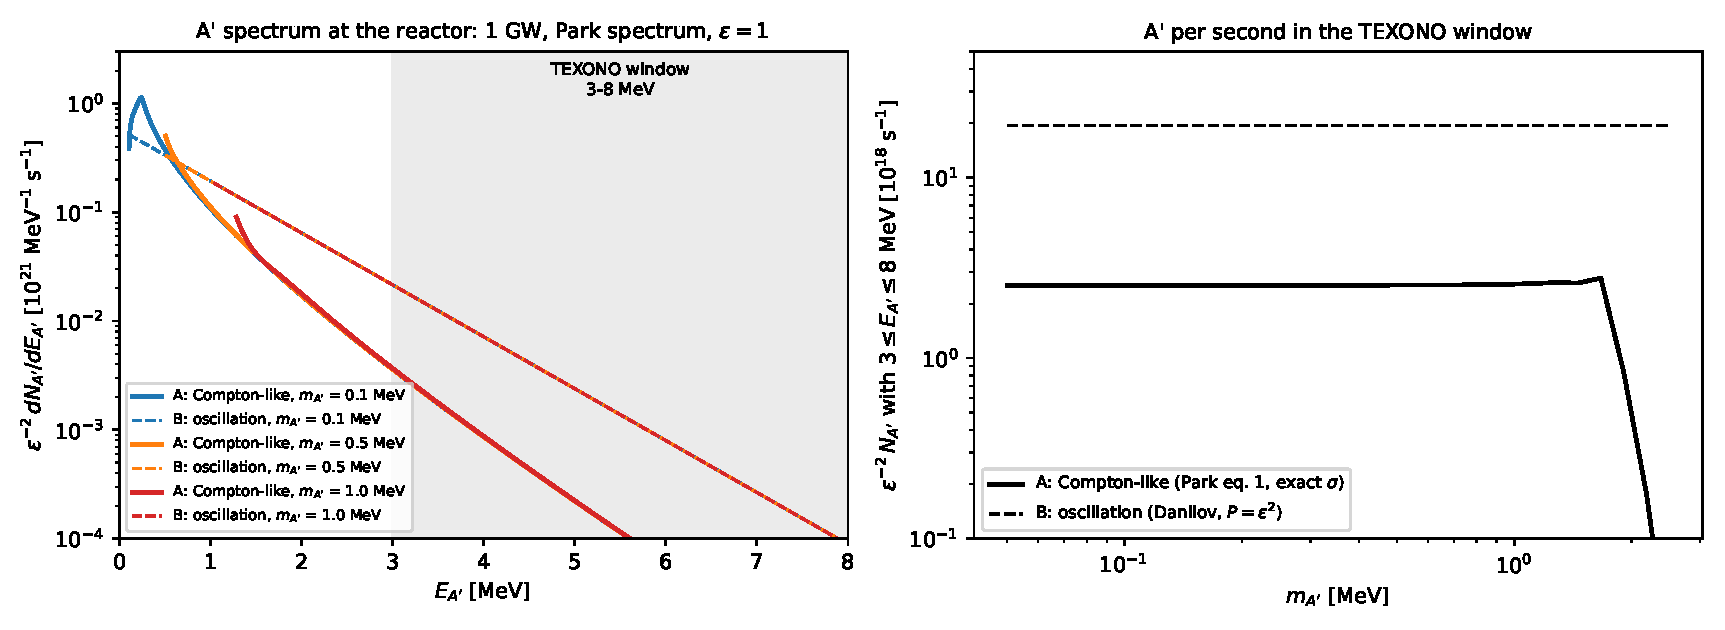
\includegraphics[width=\textwidth]{../work/fig_dN_dE_two_models.pdf}
\caption{Número esperado de $\Ap$ producidos por segundo en un reactor de 1~GW con el espectro de Park, $\eps=1$.
Izquierda: espectro $\dd\dot N_{\Ap}/\dd E_{\Ap}$ para el mecanismo A (tipo Compton, ec.~\eqref{eq:park1} con la
sección eficaz exacta, línea llena) y el mecanismo B (oscilación, ec.~\eqref{eq:danilov} con $P=\eps^2$ y
$E_{\Ap}=E_\gamma$, a trazos) para $m_{\Ap}=0.1,0.5,1$~MeV; banda gris: ventana 3--8~MeV de TEXONO. Derecha: $\Ap$ por
segundo en esa ventana en función de la masa. B supera a A por $7.7$ en la ventana; ambos son $\propto\eps^2$.}
\label{fig:two}
\end{figure}

\section{El factor de detección $2/3$}
La ec.~(6) de Park escribe $\dd\sigma_{\Ap e\to\gamma e}/\dd E_r\approx\tfrac23\eps^2\,\dd\sigma_C/\dd E_r$; Lou--Wu
ec.~(11) lo repite; Danilov et al.\ lo llaman irrelevante; el informe \emph{v3} usa $P_{X\to\gamma}\sigma_\KN$ sin $2/3$.
Calculado acá con las mismas matrices explícitas para el proceso inverso $\Ap(q)+e\to\gamma+e$, integrado sobre el
ángulo del CM, $E_{\Ap}=3$~MeV, $M=0.01$~MeV:
\begin{equation}
\frac{\sigma_T}{\eps^2\sigma_\KN}=0.99999,\qquad
\frac{\sigma_L}{\eps^2\sigma_\KN}=3\times10^{-5},\qquad
\frac{\tfrac13(2\sigma_T+\sigma_L)}{\eps^2\sigma_\KN}=0.66667 .
\end{equation}
El $2/3$ es el promedio no polarizado: dos polarizaciones transversales que dispersan como fotones y una longitudinal
que no. Aplica solo a un haz de $\Ap$ no polarizado. El haz del reactor no es no polarizado: la
oscilación/emisión directa da solo $\Ap$ transversales (Danilov: la producción longitudinal es $\propto m_X^2/E^2$), y la
producción tipo Compton, calculada acá con el vector longitudinal explícito, da una fracción longitudinal
$\sigma_L/\sigma_{\rm tot}=0.010$ en $(E,M)=(3,0.1)$~MeV, $0.195$ en $(3,0.5)$, $0.078$ en $(3,1)$, $0.211$ en $(8,1)$
(Fig.~\ref{fig:long}). La sección eficaz de detección correcta es
\begin{equation}
\sigma_{\rm det}=f_T\,\sigma_T+f_L\,\sigma_L,\qquad
\frac{\sigma_T}{\eps^2\sigma_\KN}=0.98\text{--}1.00,\quad
\frac{\sigma_L}{\eps^2\sigma_\KN}=0.02\text{--}0.31\quad (M=0.5\text{--}1,\ E_{\Ap}=3\text{--}8~{\rm MeV}),
\end{equation}
con $f_{T,L}$ las fracciones producidas. Para $M\lesssim0.1$~MeV esto es $\eps^2\sigma_\KN$ al $1\%$: factor 1, no $2/3$.
Danilov tiene razón, Park no, y la ec.~(11) de Lou--Wu es una afirmación correcta sobre un haz no polarizado aplicada a
un haz que no lo es. En $\eps$ el $2/3$ es un efecto del $10\%$ ($\eps\propto N^{-1/4}$); importa para la contabilidad,
no para el gráfico de exclusión.

\begin{figure}[t]\centering
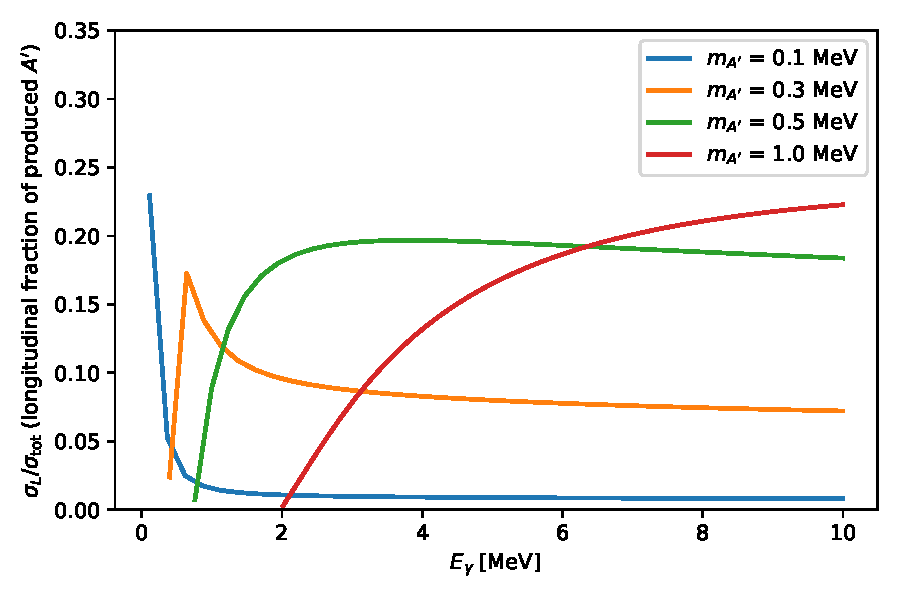
\includegraphics[width=0.62\textwidth]{../work/fig_longitudinal_fraction.pdf}
\caption{Fracción longitudinal de los $\Ap$ producidos por Compton, de la contracción explícita con $\xi_L$ integrada
sobre $[x_-,x_+]$. No es $\propto M^2/E_\gamma^2$: cerca del umbral y para $M\gtrsim0.3$~MeV es 10--25\%.}
\label{fig:long}
\end{figure}

\section{La fórmula a usar}
Para el número de $\Ap$ por unidad de energía que llegan a un detector a distancia $R$, por segundo, para
$m_{\Ap}\gg m_\gamma$ y lejos de la resonancia $m_{\Ap}\approx m_\gamma$:
\begin{equation}
\boxed{\;
\frac{\dd\Phi_{\Ap}}{\dd x}=\frac{1}{4\pi R^2}\left[\eps^2\,\frac{m_{\Ap}^4}{m_{\Ap}^4+x^2\Gamma_{\rm tot}^2}\,S_\gamma(x)\,f(x)
\;+\;\int\dd E\,S_\gamma(E)\,\frac{1}{\sigma_{\rm tot}(E)}\frac{\dd\sigma(E,x)}{\dd x}\right]
\;}
\label{eq:final}
\end{equation}
donde el primer término es la ec.~\eqref{eq:danilov} (dominante; $f(x)$ es el factor de fotones secundarios de Demidov si
el segundo término no se mantiene explícito: no contar ambos), $\dd\sigma/\dd x$ es la ec.~\eqref{eq:dsdx} con la
ec.~\eqref{eq:F}, y $\sigma_{\rm tot}$ es el total de XCOM para el material del núcleo. La tasa en el detector es entonces
$N_e T\int\dd x\,(\dd\Phi/\dd x)\,\sigma_{\rm det}(x)$ con $\sigma_{\rm det}$ como en la sección anterior. El informe
\emph{v3} implementa solo el primer término, con $\sigma_{\rm det}=\eps^2\sigma_\KN$; ese es el orden dominante correcto.
El informe \emph{v2} y Park implementan solo el segundo término; el apunte en castellano implementa el segundo
término con la sección eficaz equivocada.

Dos elecciones de normalización en \texttt{apuntes/} no son errores pero hay que declararlas: el tope de eventos de
TEXONO es $197.2$ (Park, $1.96\sigma$ a dos colas) o $195.7$ (Danilov, $95\%$ a una cola, usado por el \emph{v3}), y
Danilov lo multiplican por el factor 6 de supresión anti-Compton hasta $1174.1$ (también usado por Du et al.); el
\emph{v3} no.

\section{Qué se verificó y qué no}
\label{sec:receipt}
Verificado, con aserciones: el $|\mathcal M|^2$ de matrices explícitas contra \emph{v2}, deNiverville y Smirnov; la
identidad de Ward; el límite KN; el rango exacto y el umbral; las ecs.~(18)--(20), (40), (50), (52) del apunte y la convolución de (50) con el espectro; la primitiva
$G(b)$ del \emph{v2}; el total KN por cuadratura; las secciones eficaces inversas resueltas en polarización; los conteos
en ventana y los espectros de los dos mecanismos, incluido que la integral de la ec.~\eqref{eq:park1} sobre $E_{\Ap}$
devuelve el número de fotones; la integral de fotones de Park.

No verificado: el total de Gondolo--Raffelt (el paper no está en la carpeta; el chequeo propio del \emph{v2} queda en
$7\times10^{-14}$); el generador de Park y el código de convolución del \emph{v2} (ninguno disponible; los valores de las Figuras~1 y 2 de
arriba están leídos a ojo de los rasters, $\pm30\%$); los números de atenuación
XCOM/NIST (recordados del \emph{v2}); los Monte Carlo de Du y de Demidov; la región de resonancia
$m_{\Ap}\approx m_\gamma$; efectos de electrón ligado y transporte en el reactor; cualquier cosa de deNiverville más allá
de las ecs.~(18)--(20) y de NEON más allá de su ec.~(2).

\medskip\noindent\sloppy
Recibo de ejecución: 21 de septiembre de 2026, \texttt{work/.venv/bin/python work/check\_cross\_section.py} (numpy
2.5.2, sympy 1.12, scipy 1.18.1, Python 3 del sistema, venv con marimo 0.24.2); salida en
\texttt{work/check\_cross\_section.log}, última línea \texttt{ALL ASSERTIONS PASSED}; números en
\texttt{work/check\_cross\_section\_out.json}; figuras con \texttt{marimo export html work/figures\_cross\_section.py}.

\begin{thebibliography}{9}\small
\bibitem{park} H.~K.~Park, Phys.\ Rev.\ Lett.\ 119, 081801 (2017). \texttt{papers\_reactor\_dark\_photon/01}.
\bibitem{danilov} M.~Danilov, S.~Demidov, D.~Gorbunov, Phys.\ Rev.\ Lett.\ 122, 041801 (2019). \texttt{02}.
\bibitem{deniv} P.~deNiverville, H.-S.~Lee, Y.-M.~Lee, arXiv:2011.03276, ecs.~(18)--(20). \texttt{03}.
\bibitem{smirnov} M.~Smirnov et al., Phys.\ Rev.\ D 104, 116024 (2021), ecs.~(3)--(4). \texttt{04}.
\bibitem{du} M.~Du, J.~Liu, X.-P.~Wang, T.~Wu, Phys.\ Rev.\ D 109, 055041 (2024). \texttt{05}.
\bibitem{neon} Colaboración NEON, Phys.\ Rev.\ Lett.\ 134, 021802 (2025), ec.~(2). \texttt{06}.
\bibitem{demidov} S.~Demidov, D.~Gorbunov, A.~Polonski, arXiv:2512.17652. \texttt{07}.
\bibitem{louwu} Y.~Lou, L.~Wu, arXiv:2606.08487, ecs.~(8), (11), Ap.~A. \texttt{08}.
\end{thebibliography}
\end{document}
